% Created by tikzDevice version 0.12
% !TEX encoding = UTF-8 Unicode
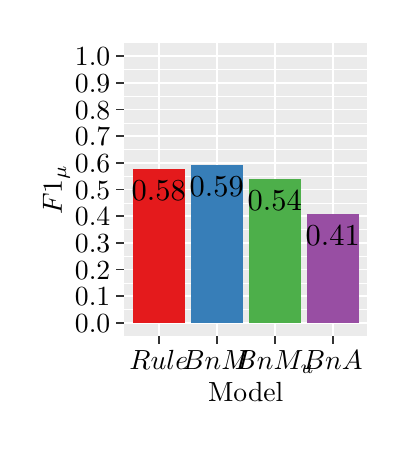
\begin{tikzpicture}[x=1pt,y=1pt]
\definecolor{fillColor}{RGB}{255,255,255}
\path[use as bounding box,fill=fillColor,fill opacity=0.00] (0,0) rectangle (128.29,142.39);
\begin{scope}
\path[clip] (  0.00,  0.00) rectangle (128.29,142.39);
\definecolor{drawColor}{RGB}{255,255,255}
\definecolor{fillColor}{RGB}{255,255,255}

\path[draw=drawColor,line width= 0.6pt,line join=round,line cap=round,fill=fillColor] (  0.00,  0.00) rectangle (128.29,142.39);
\end{scope}
\begin{scope}
\path[clip] ( 34.81, 30.86) rectangle (122.79,136.89);
\definecolor{fillColor}{gray}{0.92}

\path[fill=fillColor] ( 34.81, 30.86) rectangle (122.79,136.89);
\definecolor{drawColor}{RGB}{255,255,255}

\path[draw=drawColor,line width= 0.3pt,line join=round] ( 34.81, 40.50) --
	(122.79, 40.50);

\path[draw=drawColor,line width= 0.3pt,line join=round] ( 34.81, 50.14) --
	(122.79, 50.14);

\path[draw=drawColor,line width= 0.3pt,line join=round] ( 34.81, 59.78) --
	(122.79, 59.78);

\path[draw=drawColor,line width= 0.3pt,line join=round] ( 34.81, 69.42) --
	(122.79, 69.42);

\path[draw=drawColor,line width= 0.3pt,line join=round] ( 34.81, 79.06) --
	(122.79, 79.06);

\path[draw=drawColor,line width= 0.3pt,line join=round] ( 34.81, 88.69) --
	(122.79, 88.69);

\path[draw=drawColor,line width= 0.3pt,line join=round] ( 34.81, 98.33) --
	(122.79, 98.33);

\path[draw=drawColor,line width= 0.3pt,line join=round] ( 34.81,107.97) --
	(122.79,107.97);

\path[draw=drawColor,line width= 0.3pt,line join=round] ( 34.81,117.61) --
	(122.79,117.61);

\path[draw=drawColor,line width= 0.3pt,line join=round] ( 34.81,127.25) --
	(122.79,127.25);

\path[draw=drawColor,line width= 0.6pt,line join=round] ( 34.81, 35.68) --
	(122.79, 35.68);

\path[draw=drawColor,line width= 0.6pt,line join=round] ( 34.81, 45.32) --
	(122.79, 45.32);

\path[draw=drawColor,line width= 0.6pt,line join=round] ( 34.81, 54.96) --
	(122.79, 54.96);

\path[draw=drawColor,line width= 0.6pt,line join=round] ( 34.81, 64.60) --
	(122.79, 64.60);

\path[draw=drawColor,line width= 0.6pt,line join=round] ( 34.81, 74.24) --
	(122.79, 74.24);

\path[draw=drawColor,line width= 0.6pt,line join=round] ( 34.81, 83.87) --
	(122.79, 83.87);

\path[draw=drawColor,line width= 0.6pt,line join=round] ( 34.81, 93.51) --
	(122.79, 93.51);

\path[draw=drawColor,line width= 0.6pt,line join=round] ( 34.81,103.15) --
	(122.79,103.15);

\path[draw=drawColor,line width= 0.6pt,line join=round] ( 34.81,112.79) --
	(122.79,112.79);

\path[draw=drawColor,line width= 0.6pt,line join=round] ( 34.81,122.43) --
	(122.79,122.43);

\path[draw=drawColor,line width= 0.6pt,line join=round] ( 34.81,132.07) --
	(122.79,132.07);

\path[draw=drawColor,line width= 0.6pt,line join=round] ( 47.38, 30.86) --
	( 47.38,136.89);

\path[draw=drawColor,line width= 0.6pt,line join=round] ( 68.32, 30.86) --
	( 68.32,136.89);

\path[draw=drawColor,line width= 0.6pt,line join=round] ( 89.27, 30.86) --
	( 89.27,136.89);

\path[draw=drawColor,line width= 0.6pt,line join=round] (110.22, 30.86) --
	(110.22,136.89);
\definecolor{fillColor}{RGB}{228,26,28}

\path[fill=fillColor] ( 37.95, 35.68) rectangle ( 56.80, 91.21);
\definecolor{fillColor}{RGB}{55,126,184}

\path[fill=fillColor] ( 58.90, 35.68) rectangle ( 77.75, 92.63);
\definecolor{fillColor}{RGB}{77,175,74}

\path[fill=fillColor] ( 79.85, 35.68) rectangle ( 98.70, 87.76);
\definecolor{fillColor}{RGB}{152,78,163}

\path[fill=fillColor] (100.79, 35.68) rectangle (119.65, 75.15);
\definecolor{drawColor}{RGB}{0,0,0}

\node[text=drawColor,anchor=base,inner sep=0pt, outer sep=0pt, scale=  1.10] at (110.22, 63.75) {0.41};

\node[text=drawColor,anchor=base,inner sep=0pt, outer sep=0pt, scale=  1.10] at ( 89.27, 76.36) {0.54};

\node[text=drawColor,anchor=base,inner sep=0pt, outer sep=0pt, scale=  1.10] at ( 68.32, 81.23) {0.59};

\node[text=drawColor,anchor=base,inner sep=0pt, outer sep=0pt, scale=  1.10] at ( 47.38, 79.81) {0.58};
\end{scope}
\begin{scope}
\path[clip] (  0.00,  0.00) rectangle (128.29,142.39);
\definecolor{drawColor}{RGB}{0,0,0}

\node[text=drawColor,anchor=base east,inner sep=0pt, outer sep=0pt, scale=  1.00] at ( 29.86, 32.24) {0.0};

\node[text=drawColor,anchor=base east,inner sep=0pt, outer sep=0pt, scale=  1.00] at ( 29.86, 41.88) {0.1};

\node[text=drawColor,anchor=base east,inner sep=0pt, outer sep=0pt, scale=  1.00] at ( 29.86, 51.52) {0.2};

\node[text=drawColor,anchor=base east,inner sep=0pt, outer sep=0pt, scale=  1.00] at ( 29.86, 61.15) {0.3};

\node[text=drawColor,anchor=base east,inner sep=0pt, outer sep=0pt, scale=  1.00] at ( 29.86, 70.79) {0.4};

\node[text=drawColor,anchor=base east,inner sep=0pt, outer sep=0pt, scale=  1.00] at ( 29.86, 80.43) {0.5};

\node[text=drawColor,anchor=base east,inner sep=0pt, outer sep=0pt, scale=  1.00] at ( 29.86, 90.07) {0.6};

\node[text=drawColor,anchor=base east,inner sep=0pt, outer sep=0pt, scale=  1.00] at ( 29.86, 99.71) {0.7};

\node[text=drawColor,anchor=base east,inner sep=0pt, outer sep=0pt, scale=  1.00] at ( 29.86,109.35) {0.8};

\node[text=drawColor,anchor=base east,inner sep=0pt, outer sep=0pt, scale=  1.00] at ( 29.86,118.99) {0.9};

\node[text=drawColor,anchor=base east,inner sep=0pt, outer sep=0pt, scale=  1.00] at ( 29.86,128.62) {1.0};
\end{scope}
\begin{scope}
\path[clip] (  0.00,  0.00) rectangle (128.29,142.39);
\definecolor{drawColor}{gray}{0.20}

\path[draw=drawColor,line width= 0.6pt,line join=round] ( 32.06, 35.68) --
	( 34.81, 35.68);

\path[draw=drawColor,line width= 0.6pt,line join=round] ( 32.06, 45.32) --
	( 34.81, 45.32);

\path[draw=drawColor,line width= 0.6pt,line join=round] ( 32.06, 54.96) --
	( 34.81, 54.96);

\path[draw=drawColor,line width= 0.6pt,line join=round] ( 32.06, 64.60) --
	( 34.81, 64.60);

\path[draw=drawColor,line width= 0.6pt,line join=round] ( 32.06, 74.24) --
	( 34.81, 74.24);

\path[draw=drawColor,line width= 0.6pt,line join=round] ( 32.06, 83.87) --
	( 34.81, 83.87);

\path[draw=drawColor,line width= 0.6pt,line join=round] ( 32.06, 93.51) --
	( 34.81, 93.51);

\path[draw=drawColor,line width= 0.6pt,line join=round] ( 32.06,103.15) --
	( 34.81,103.15);

\path[draw=drawColor,line width= 0.6pt,line join=round] ( 32.06,112.79) --
	( 34.81,112.79);

\path[draw=drawColor,line width= 0.6pt,line join=round] ( 32.06,122.43) --
	( 34.81,122.43);

\path[draw=drawColor,line width= 0.6pt,line join=round] ( 32.06,132.07) --
	( 34.81,132.07);
\end{scope}
\begin{scope}
\path[clip] (  0.00,  0.00) rectangle (128.29,142.39);
\definecolor{drawColor}{gray}{0.20}

\path[draw=drawColor,line width= 0.6pt,line join=round] ( 47.38, 28.11) --
	( 47.38, 30.86);

\path[draw=drawColor,line width= 0.6pt,line join=round] ( 68.32, 28.11) --
	( 68.32, 30.86);

\path[draw=drawColor,line width= 0.6pt,line join=round] ( 89.27, 28.11) --
	( 89.27, 30.86);

\path[draw=drawColor,line width= 0.6pt,line join=round] (110.22, 28.11) --
	(110.22, 30.86);
\end{scope}
\begin{scope}
\path[clip] (  0.00,  0.00) rectangle (128.29,142.39);
\definecolor{drawColor}{RGB}{0,0,0}

\node[text=drawColor,anchor=base,inner sep=0pt, outer sep=0pt, scale=  1.00] at ( 47.38, 19.03) {\(Rule\)};

\node[text=drawColor,anchor=base,inner sep=0pt, outer sep=0pt, scale=  1.00] at ( 68.32, 19.03) {\(BnM\)};

\node[text=drawColor,anchor=base,inner sep=0pt, outer sep=0pt, scale=  1.00] at ( 89.27, 19.03) {\(BnM_u\)};

\node[text=drawColor,anchor=base,inner sep=0pt, outer sep=0pt, scale=  1.00] at (110.22, 19.03) {\(BnA\)};
\end{scope}
\begin{scope}
\path[clip] (  0.00,  0.00) rectangle (128.29,142.39);
\definecolor{drawColor}{RGB}{0,0,0}

\node[text=drawColor,anchor=base,inner sep=0pt, outer sep=0pt, scale=  1.00] at ( 78.80,  7.44) {Model};
\end{scope}
\begin{scope}
\path[clip] (  0.00,  0.00) rectangle (128.29,142.39);
\definecolor{drawColor}{RGB}{0,0,0}

\node[text=drawColor,rotate= 90.00,anchor=base,inner sep=0pt, outer sep=0pt, scale=  1.00] at ( 12.39, 83.87) {\(F1_\mu\)};
\end{scope}
\end{tikzpicture}
